\documentclass[12pt,letterpaper]{article}
%%% LuaLaTex
\usepackage{fontspec}
\usepackage{amsmath}% if desired
\usepackage{unicode-math}
\renewcommand{\boldsymbol}{\symbf}

\setmainfont{TeX Gyre Pagella}[
Numbers	=	{OldStyle, Proportional},
Ligatures	=	TeX,
%Script=Arabic
%Contextuals = WordFinal,	
]
\setsansfont{TeX Gyre Adventor}[
Numbers	=	{OldStyle, Proportional},
Ligatures	=	TeX,
Scale=MatchLowercase]
\setmonofont{Inconsolata}[
Scale = MatchLowercase, 
Ligatures = TeX,
]
\setmathfont{XITS Math}
\setmathfont[range=it->up]{Neo Euler}
\setmathfont[range=up/{num}]{Neo Euler}
\newfontface{\andm}{Andale Mono}
\newfontface{\babm}{BabelStone Mayan Numerals}%{Symbola}
\newfontface{\mayanumerals}{BabelStone Mayan Numerals}
\newfontface{\charis}{Charis SIL}%{Gentium Plus}
\newfontface{\charisbf}{Charis SIL Bold}%{Charis SIL}
%\newfontface{\palarab}{PalatinoLTArabic}%{Gentium Plus}
%%%%%%%%%%%%
\linespread{1.05}% Palatino needs more leading (space between lines) {1.01} {1.08}
%\usepackage{ucs}
\usepackage[spanish,mexico]{babel}
%\usepackage{amsmath}
%\usepackage{amsfonts}
%\usepackage{amssymb}
%\usepackage{makeidx}
\usepackage[format=hang,font=small,labelfont=bf,labelsep=quad]{caption}
\usepackage{xcolor}
\usepackage{graphicx}
\usepackage[useregional]{datetime2}
\usepackage{fancyhdr}
\usepackage{tikz}
\usepackage[colorlinks=true,urlcolor=brown]{hyperref}
% % % %Geometry
\usepackage{geometry}%\usepackage[showframe]{geometry}
%\usepackage{layout}
\setlength{\voffset}{-0.7in}
\setlength{\headsep}{10pt}
\setlength{\textheight}{10.5in}
%\usepackage{coloremoji}
\usepackage{wasysym} %emoticons :)
\newcommand{\LuaLaTeX}{L\kern-0.25em\raise0.5ex\hbox{\tiny U}\kern-0.04em\raise0.5ex\hbox{\tiny A}\kern-0.05em\LaTeX}
\newcommand{\fej}{\relax\hfill\ifmmode{\lower.5ex\hbox{{\textcolor{blue}{\LARGE\smiley al 15pt}}}}\else\lower.5ex\hbox{{\textcolor{blue}{\LARGE \smiley}}}}  % Smiley emoticon :)
%\newcommand{\fej}{\relax\hfill\ifmmode{\lower.5ex\hbox{{\textcolor{blue}{\LARGE\smiley}}}}\else\lower.5ex\hbox{{\textcolor{blue}{\LARGE \smiley}}}}  % Smiley emoticon :)
\author{\textsc{Manuel López Mateos}}
% % % % % % % Para usar título, autor y fecha por separado.
\makeatletter
\let\newtitle\@title
\let\elautor\@author
\let\newdate\@date
\makeatother
%
%
% % % % Enviroments
\newenvironment{definition}[1][Definición.]{\begin{trivlist}
\item[\hskip \labelsep {\bfseries #1}]}{\end{trivlist}}
% % % % % % % % % % % %
%
% % % % % % % % Headers
\pagestyle{fancy}
\fancyhf{}
\rhead{\color{olive}\hfill \DTMnow}
\lhead{\color{olive}\elautor}
\cfoot{\thepage}
\renewcommand{\headrule}{\color{olive}\hrule}
\newcommand{\R}{\relax\ifmmode\mathbb{R}\else${\mathbb{R}}$\fi}
%\rfoot{}
% % % % % % %
\begin{document} %\layout
%\noindent{\color{purple} \elautor \hfill \DTMnow
%\smallskip
%
%\hrule}
\bigskip 

\noindent Dado un triángulo en el plano $\R^2$, por ejemplo, el definido por los puntos $A=(-2,4)$, $B=(-3,-2)$ y $C=(6,-1)$ hay varias rectas y puntos asociados a él, se les conoce como \emph{rectas notables} y \emph{puntos notables} del triángulo. Estas rectas son las \emph{\color{blue}mediatrices}, las \emph{\color{orange}medianas} y las \emph{\color{green}alturas}; en la figura ilustramos las correspondientes al lado $a$, opuesto al vértice $A$.
\begin{figure}[ht]
	\centering
	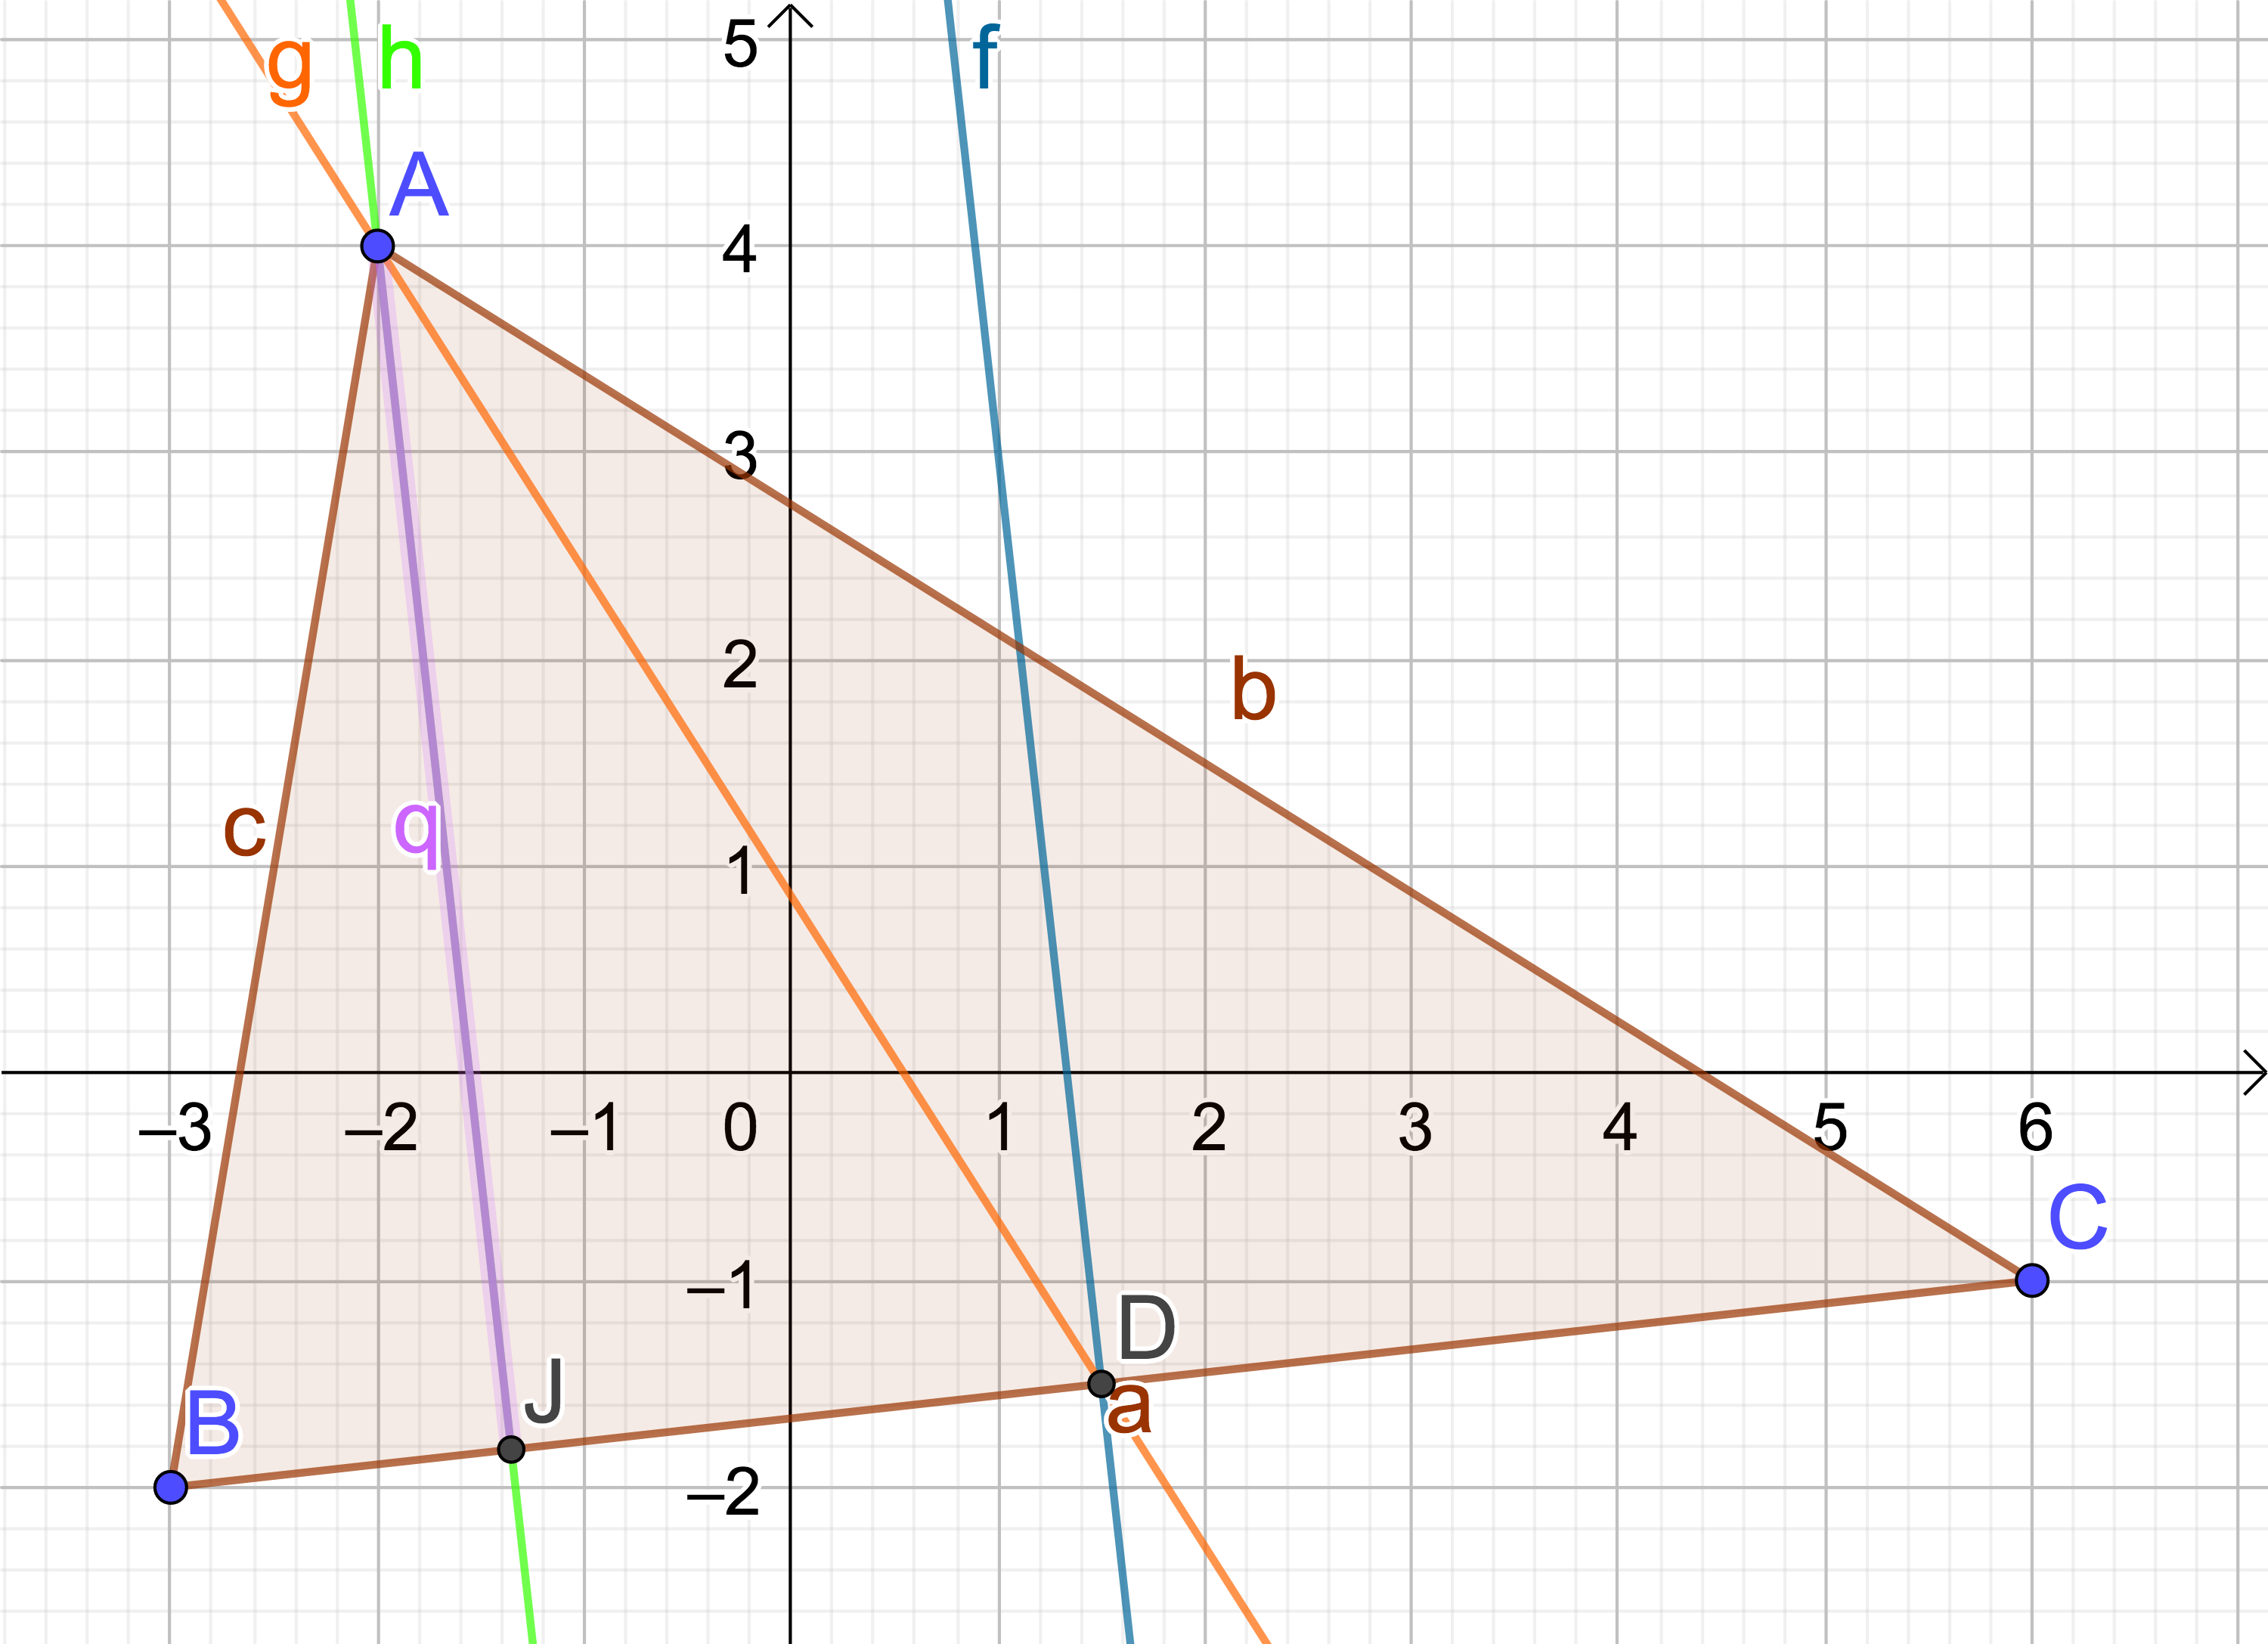
\includegraphics[scale=0.6]{img/MedtrMedAlt-Triangc.png}
	\caption{\emph{Mediatriz} de $a$ (en azul), \emph{Mediana} de $a$ desde $A$ (en anaranjado) y \emph{Altura} que pasa por $A$ (segmento $\overline{AJ}$ en púrpura).}\label{fig:metmedalt}
\end{figure}

Las \textbf{\color{purple}mediatrices} de los lados de un triángulo, son las rectas \emph{perpendiculares} a cada lado que pasan por su \emph{punto medio}. Así, la \emph{mediatriz} del lado $a$ es la perpendicular a la recta que lo contiene, que pasa por $D$, el punto medio del lado $a$.

Las \textbf{\color{purple}medianas} de un triángulo son las rectas que pasan por un \emph{vértice} y por el \emph{punto medio} del lado opuesto. Así, la \emph{mediana} que pasa por el vértice $A$, también pasa por $D$, el punto medio del lado $a$

Las \textbf{\color{purple}alturas} de un triángulo son segmentos que pasan por un vértice y la base de la perpendicular al lado opuesto. Así, la \emph{altura} correspondiente al vértice $A$ es el segmento $\overline{AJ}$, donde $J$ es la base de la perpendicular al lado $a$, que pasa por $A$. 
\smallskip

Las \emph{tres} \emph{mediatrices} se \emph{\color{purple}intersecan} en un punto, llamado \textbf{\color{purple}circuncentro} del triángulo.

Las \emph{tres} \emph{medianas} se \emph{\color{purple}intersecan} en un punto, llamado \textbf{\color{purple}baricentro}, \textbf{\color{purple}centroide} o \textbf{\color{purple}centro de gravedad} del triángulo.

Las \emph{tres} \emph{alturas} se \emph{\color{purple}intersecan} en un punto, llamado \textbf{\color{purple}ortocentro} del triángulo.
\smallskip

Los tres puntos, \emph{circuncentro}, \emph{baricentro} y \emph{ortocentro}, son colineales. La recta que los contiene se llama la \textbf{\color{purple}recta de Euler}. 
\begin{figure}[ht]
	\centering
	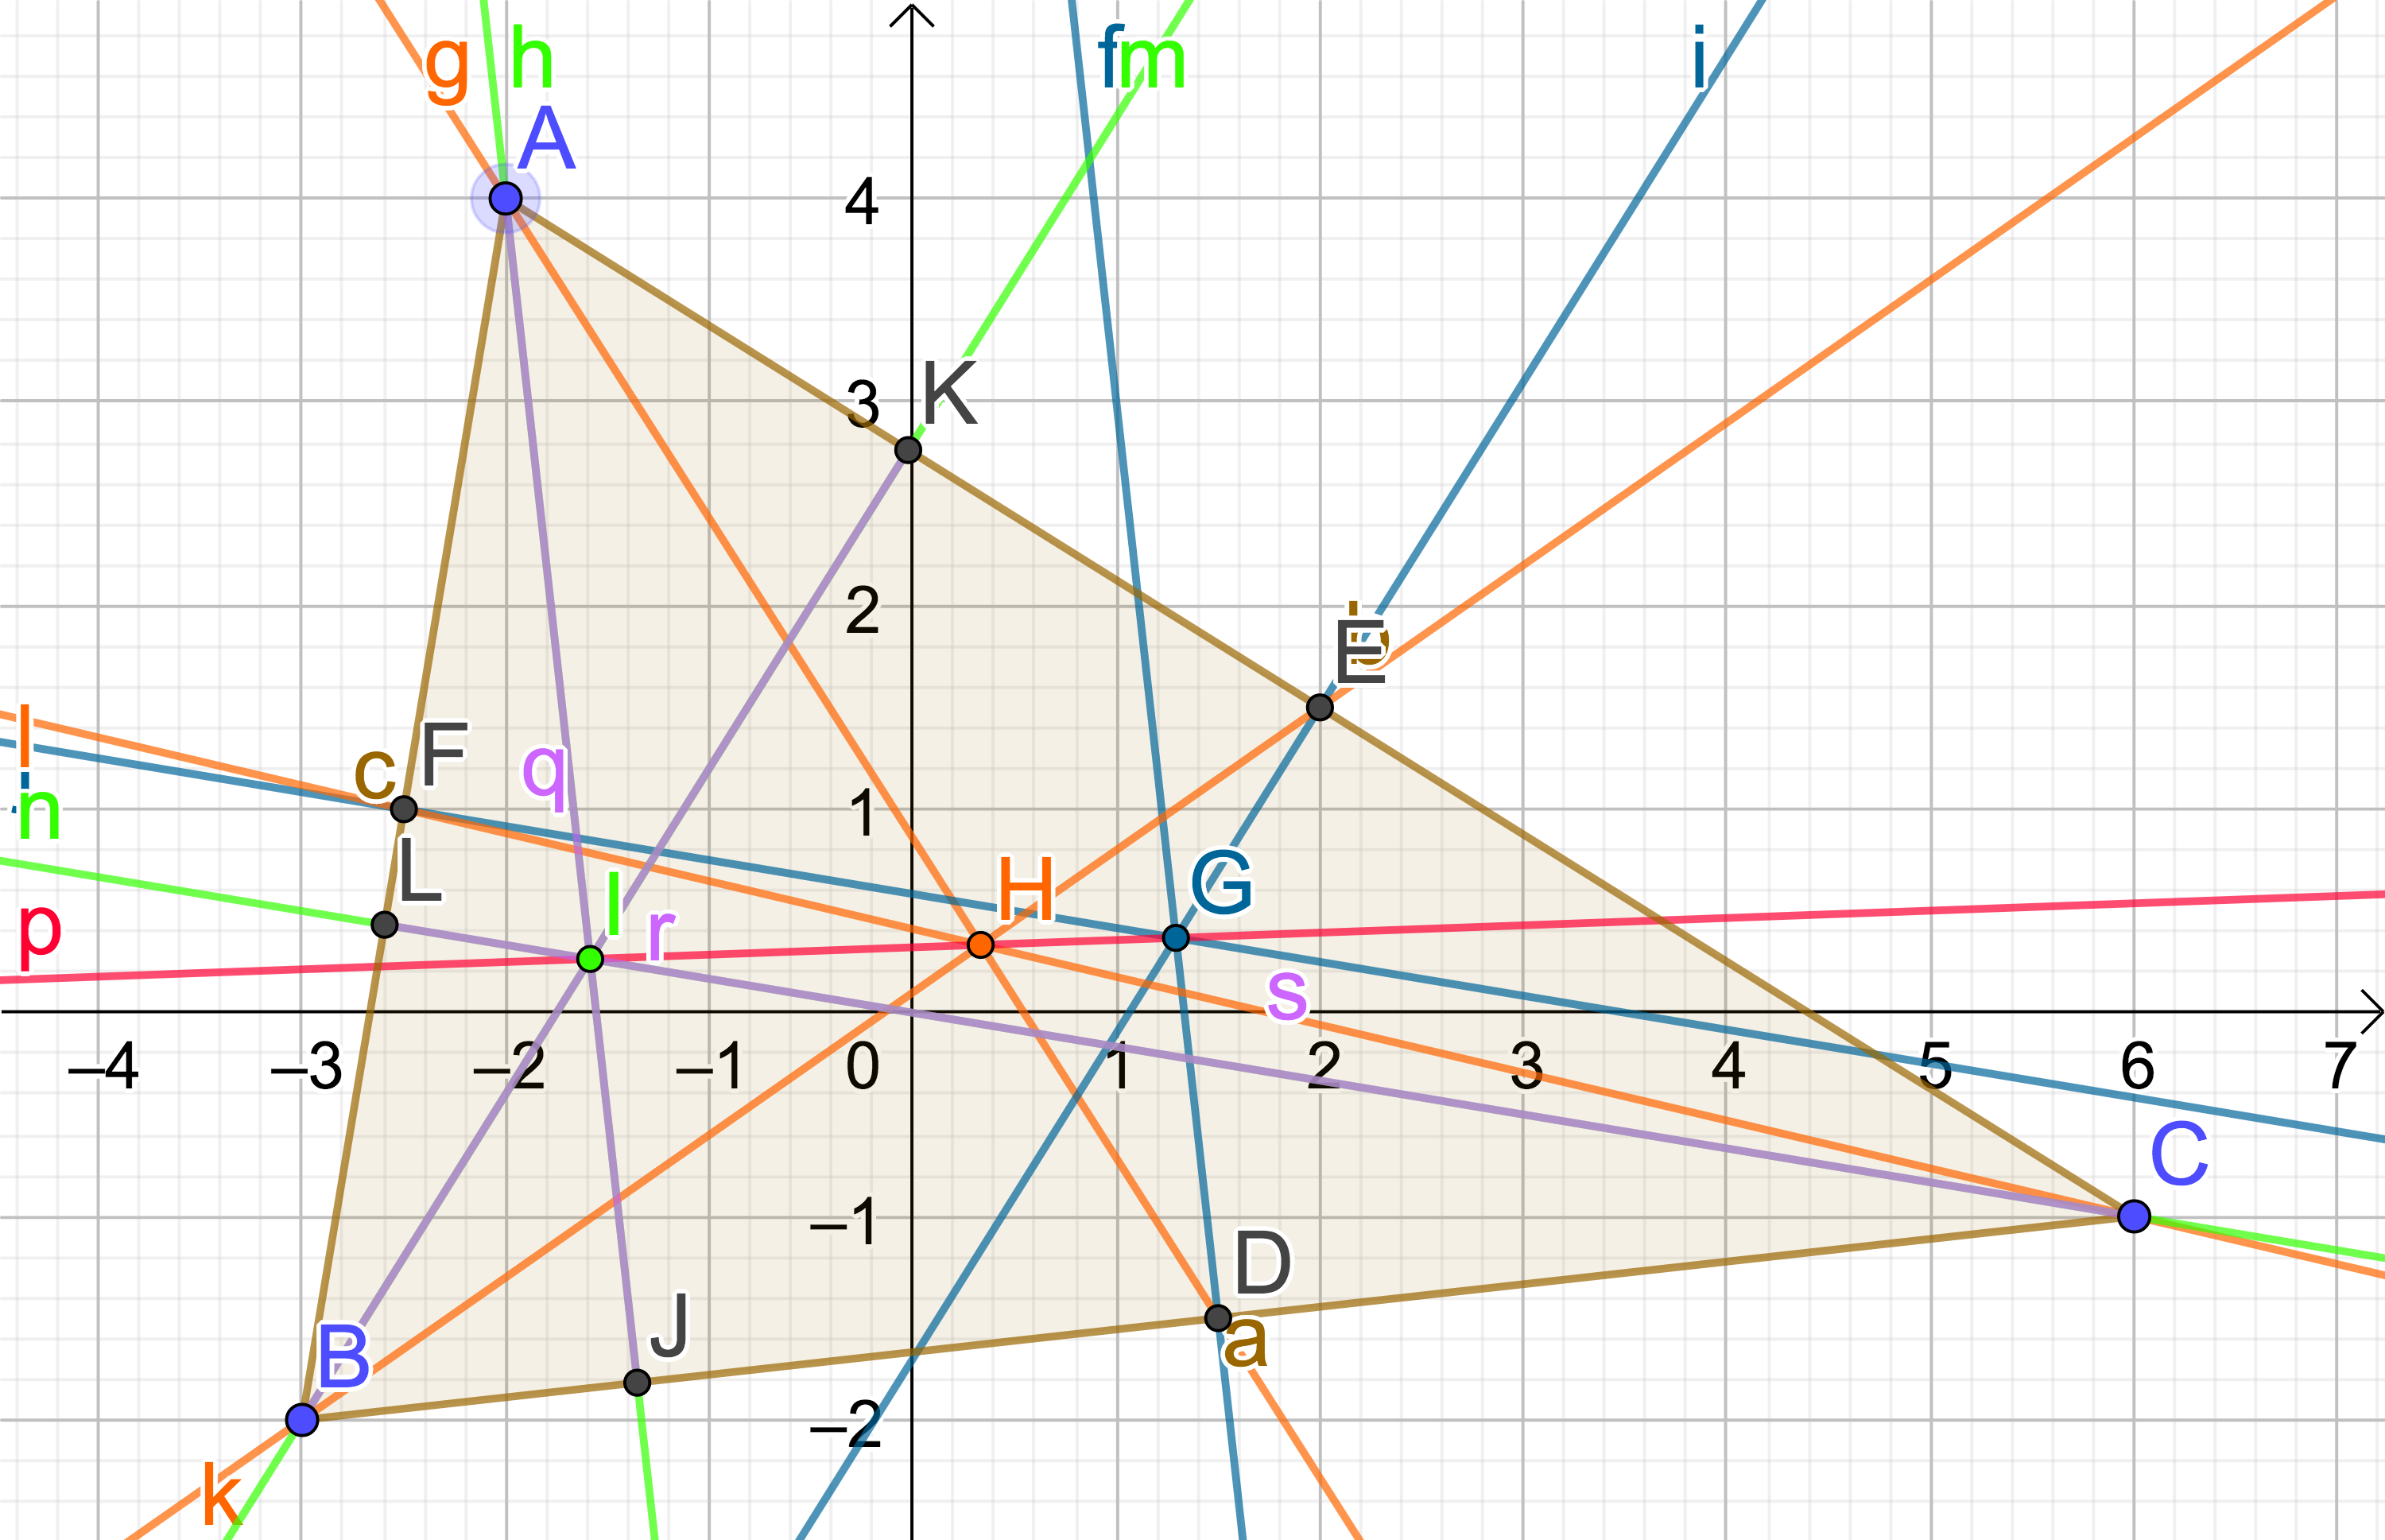
\includegraphics[scale=0.6]{img/CircBarOrt-Triangc.png}
	\caption{En rojo la recta $p$ que pasa por los puntos $G$, $H$ e $I$.}\label{fig:circbarort}
\end{figure}

\vfill 

\begin{center}
	\texttt{\color{brown}Mueve los vértices en:}\enspace \url{https://www.geogebra.org/classic/mdxd4g6a}
\end{center}

\begin{center}
	{\footnotesize\color{olive} Esta hoja se formó con el sistema \LuaLaTeX. La gráfica con \textsc{Geogebra}.}
\end{center}
\end{document}